\setchapterpreamble[u]{\margintoc}
\chapter{Generation of hyperspectral point clouds}
\labch{hyperspectral_point_clouds}
\label{sec:hyperspectral_point_clouds}

\section*{About this chapter}

This chapter describes the efficient generation of hyperspectral point clouds as the last step in the enrichment of large \acrshort{rgb} point clouds, using images collected by a push broom hyperspectral sensor. To this end, a \acrshort{gpgpu} workflow for the generation, compression and rendering of dense hyperspectral point clouds is proposed. It is capable of integrating hyperspectral images into 3D models acquired by \acrshort{lidar} or estimated with photogrammetry. Figure \ref{fig:hyper_summary} shows the main steps of this approach.

Firstly, the input \acrshort{rgb} point cloud is obtained with photogrammetry. Then, hyperspectral images are geometrically corrected and aligned among them with an \acrshort{rgb} orthomosaic helping to find common features. Therefore, hyperspectral data can be subsequently projected into the 3D point cloud using the \acrshort{gpu} to retrieve which 3D point is visible for each hyperspectral pixel. Furthermore, the rendering of large hyperspectral datasets has not been previously addressed and thus an accelerated rendering approach is proposed to tackle low performance in the visualization. Similarly, the data is compressed by partly following the work of Graciano et al. \cite{graciano_quadstack_2021} to obtain a low memory footprint while also aiming at providing a compressed representation suitable for rendering. As a result, the obtained point clouds help in studying the geometrical and hyperspectral features of natural and man-made materials in the real world.

\section{On the reconstruction of hyperspectral point clouds}

Sensors which are typically mounted on \acrshort{uas}s bring the opportunity to collect hyperspectral surface samples from multiple viewpoints. Thus, light and material interactions of real objects can be captured with a notable spatial resolution. However, the generation of 3D hyperspectral point clouds still poses challenges due to the high geometric distortions in hyperspectral swaths. Most of the current solutions use integrated \acrshort{lidar} and hyperspectral detectors, though these present several limitations as a result of errors derived from inertial measurements and the spatial resolution of \acrshort{lidar}. 

The realistic modelling of material appearance has been widely studied in Computer Graphics. The exploration of hyperspectral imaging opens the possibility to study the material's response beyond the human visible range. Recent work is presented for the acquisition of hyperspectral data through a goniophotometer and modelling of \acrshort{brdf}s from the collected data. These advances lead us toward the generation of real-world material databases, which are highly used for rendering photorealistic scenes, virtual interior design in architecture, the game industry, etc. Also, the use of hyperspectral sensors mounted in \acrshort{uas}s brings up new opportunities to explore high-resolution spectral analysis. It enables observing light-material interactions from multiple viewpoints in a large number of bands that help to characterize a wide range of real-world surfaces. Besides geometric features, studying the hyperspectral data distribution from reconstructed surfaces helps us to approach non-trivial tasks such as the modelling of specularities, interreflections, transparencies, or subsurface scattering under variable and general observation conditions. 

In the last few years, novel solutions have been proposed relying on the mechanical integration of \acrshort{lidar} sensors and hyperspectral cameras for the generation of 3D spectral data. Despite the progress made in the fusion of multiple \acrshort{uas}-based data sources, to our knowledge, there does not exist a solution capable of automatically enriching 3D point clouds with hyperspectral information. 

\begin{figure*}[bt]
    \centering
    \includegraphics[width=\linewidth]{figs/hyper_point_cloud/overview.png}
	\caption{The overall approach proposed for the generation of 3D hyperspectral point clouds. The starting point cloud is first sorted and shuffled to enhance its rendering. Hyperspectral swaths are then corrected and fused to build an orthomosaic. This result is projected into the \acrshort{rgb} point cloud, previously voxelized to obtain the visible points. The hypercube is then compressed according to a stack-based representation. }
	\label{fig:hyper_summary}
\end{figure*}

\section{Hyperspectral alignment and rectification}

Pushbroom hyperspectral sensors provide high spectral resolution data, but the acquisition mechanism leads to the collection of multiple hyperspectral swaths that present high geometric distortions, which is one of the main challenges in hyperspectral processing. Thus, the first required step is to correct these distortions, which is a time-consuming and manual task that can be solved with commercial software. Otherwise, Jurado et al. \cite{jurado_efficient_2021} proposed an automatized pipeline based on the iterative matching of hyperspectral swaths with an \acrshort{rgb} orthomosaic. This algorithm was replicated in this chapter to correct the geometrical distortions. A brief description of this approach is following presented to make this a self-contained work.

The steps for the generation of hyperspectral orthomosaics by aligning hyperspectral swaths are 1) image subdivision, 2) feature detection, 3) matching and calculation of a homography matrix, 4) image transformation, and 5) validation. Firstly, each hyperspectral swath is subdivided into multiple fragments since distortions vary through the $Y$-axis of the images. Second, the feature detection phase is performed to collect keypoints visible in multiple hyperspectral fragments and the \acrshort{rgb} orthophoto using the \acrshort{orb} feature descriptor. The likelihood of the found matches is evaluated with the Hamming distance \cite{norouzi_hamming_2012}. Then, the homography matrix is estimated in order to transform every pixel from the hyperspectral fragments, thus enabling a better alignment with the reference \acrshort{rgb} orthomosaic. A homography matrix is considered valid if the alignment error is below five pixels. To this end, the accuracy of the alignment is measured using a validation mask for each image, where control points (\acrshort{cp}) are represented with different colours. Each one was located in meaningful places within the study area, such as corners and objects that could be easily recognized in hyperspectral and \acrshort{rgb} imagery. Then, the method is capable of registering the visible markers within each fragment. Accordingly, the estimated homography was applied and the Euclidean distance was calculated for every projected position of the \acrshort{cp}s and its corresponding pixel in the \acrshort{rgb} orthomosaic. If the error was above the proposed threshold, the height of the fragment was reduced until finding an appropriate estimation or reaching the maximum number of possible subdivisions.

\section{Generation of hyperspectral orthomosaics}

Once hyperspectral swaths are corrected and aligned with \acrshort{rgb} imagery, both datasets overlap in the \acrshort{utm} coordinate system. Instead of using individual swaths in later stages, these can be merged into a single hyperspectral orthomosaic that can be efficiently sampled from a point cloud. Firstly, the offset and size of each swath are represented in \acrshort{utm}, and thus the size of the resulting hyperspectral orthomosaic is calculated by combining the 2D \acrshort{aabb} of every swath. Then, each hyperspectral pixel can be mapped to a pixel of the resulting orthomosaic. 

Radiance observations may vary among the hyperspectral swaths and the values projected in a single pixel may differ one from another. These radiometric differences have been previously revised while generating thermographic point clouds and are derived from acquisition conditions and errors induced by sensors (e.g., the striping phenomenon) \cite{pu_hyperspectral_2017}, among others. However, this chapter is not aimed at solving systematic errors which can be partially removed as a post-processing task. Instead, penalty functions were used as previously explained to obtain the most accurate aggregated radiance value, or at least, that which minimizes the dissimilarity from the initial samples. 

\begin{figure}[bt]
    \centering
    \includegraphics[width=.97\linewidth]{figs/hyper_point_cloud/orthomosaic.png}
	\caption{\acrshort{rgb} hyperspectral swaths and the reconstructed orthomosaic using penalty-based functions (green wavelength). }
	\label{fig:hyper_band_fusion}
\end{figure}

\begin{marginfigure}[.2cm]
    \centering
    \includegraphics[width=\linewidth]{figs/hyper_point_cloud/aggregation_operator.png}
	\caption{Overview of the aggregation procedure in the \acrshort{gpu}. }
	\label{fig:hyper_aggregation_insight}
\end{marginfigure}
The fusion of hyperspectral swaths was performed in the \acrshort{gpu} following the workflow in Figure \ref{fig:hyper_aggregation_insight}. Therefore, the hyperspectral orthomosaic is rapidly constructed to generate a result such as the one depicted in Figure \ref{fig:hyper_band_fusion}. The workflow is split into several stages according to the definition of penalty functions, with the complete procedure being iterated for each hyperspectral layer and orthomosaic. Firstly, aggregation outputs are computed for every hyperspectral layer and stored in a \acrshort{ssbo}. Some of these aggregations are entirely solved at the end of this stage, e.g., $\max$ and $\min$, while mean-based aggregations require an additional stage and thus were solved at the start of the following distance-measuring stage. Then, images must be iterated again to compute the result of local penalty functions ($P$) whose error is accumulated per aggregation operator, once again, storing it in an \acrshort{ssbo}. The last stage is aimed at selecting the operator that minimizes the dissimilarity to finish the construction of the hyperspectral orthomosaic (see Figure \ref{fig:hyper_aggregation_selection}). 

\begin{figure}[hbt]
    \centering
    \includegraphics[width=\linewidth]{figs/hyper_point_cloud/aggregation_selection.png}
	\caption{Point cloud rendered according to the selected aggregation operator for red (a) and green (b) wavelengths. The operator used in non-overlapped areas is irrelevant (indeed, it is the first one: $\max$). }
	\label{fig:hyper_aggregation_selection}
\end{figure}

For optimization purposes, hyperspectral images were represented as \verb|uint8_t| values that work as a rendering-based discretization of the starting radiometric resolution (in the order of $2^x$). On the other hand, aggregation buffers were allocated using the \verb|uint| data type since some operators require the sum and product of radiance samples from multiple swaths. This procedure is performed band-wise since the optimal aggregation may vary among different wavelengths. Penalty functions were implemented as subroutines, and therefore these can be easily modified in real time.

\section{Projection of hyperspectral orthomosaics}

The next stage is to project the hyperspectral orthomosaic into a 3D point cloud placed positioned in the \acrshort{utm} coordinate system. The input point cloud was reconstructed with \acrshort{sfm} using \acrshort{rgb} imagery, which led to a dense \acrshort{rgb} point cloud. On the other hand, hyperspectral swaths were acquired with a \textit{nadir} forward vector which, together with the limited scanning spatial resolution, leads to a slightly different projection that does not require occlusion checks. Instead, the point cloud will be generated as a heightfield, i.e., a 2.5D point cloud whose dimensionality depends on the hyperspectral resolution. Figure \ref{fig:hyper_voxelization} depicts the heightfield of an \acrshort{rgb} point cloud rendered with uniform colour.

\begin{marginfigure}[.1cm]
    \centering
    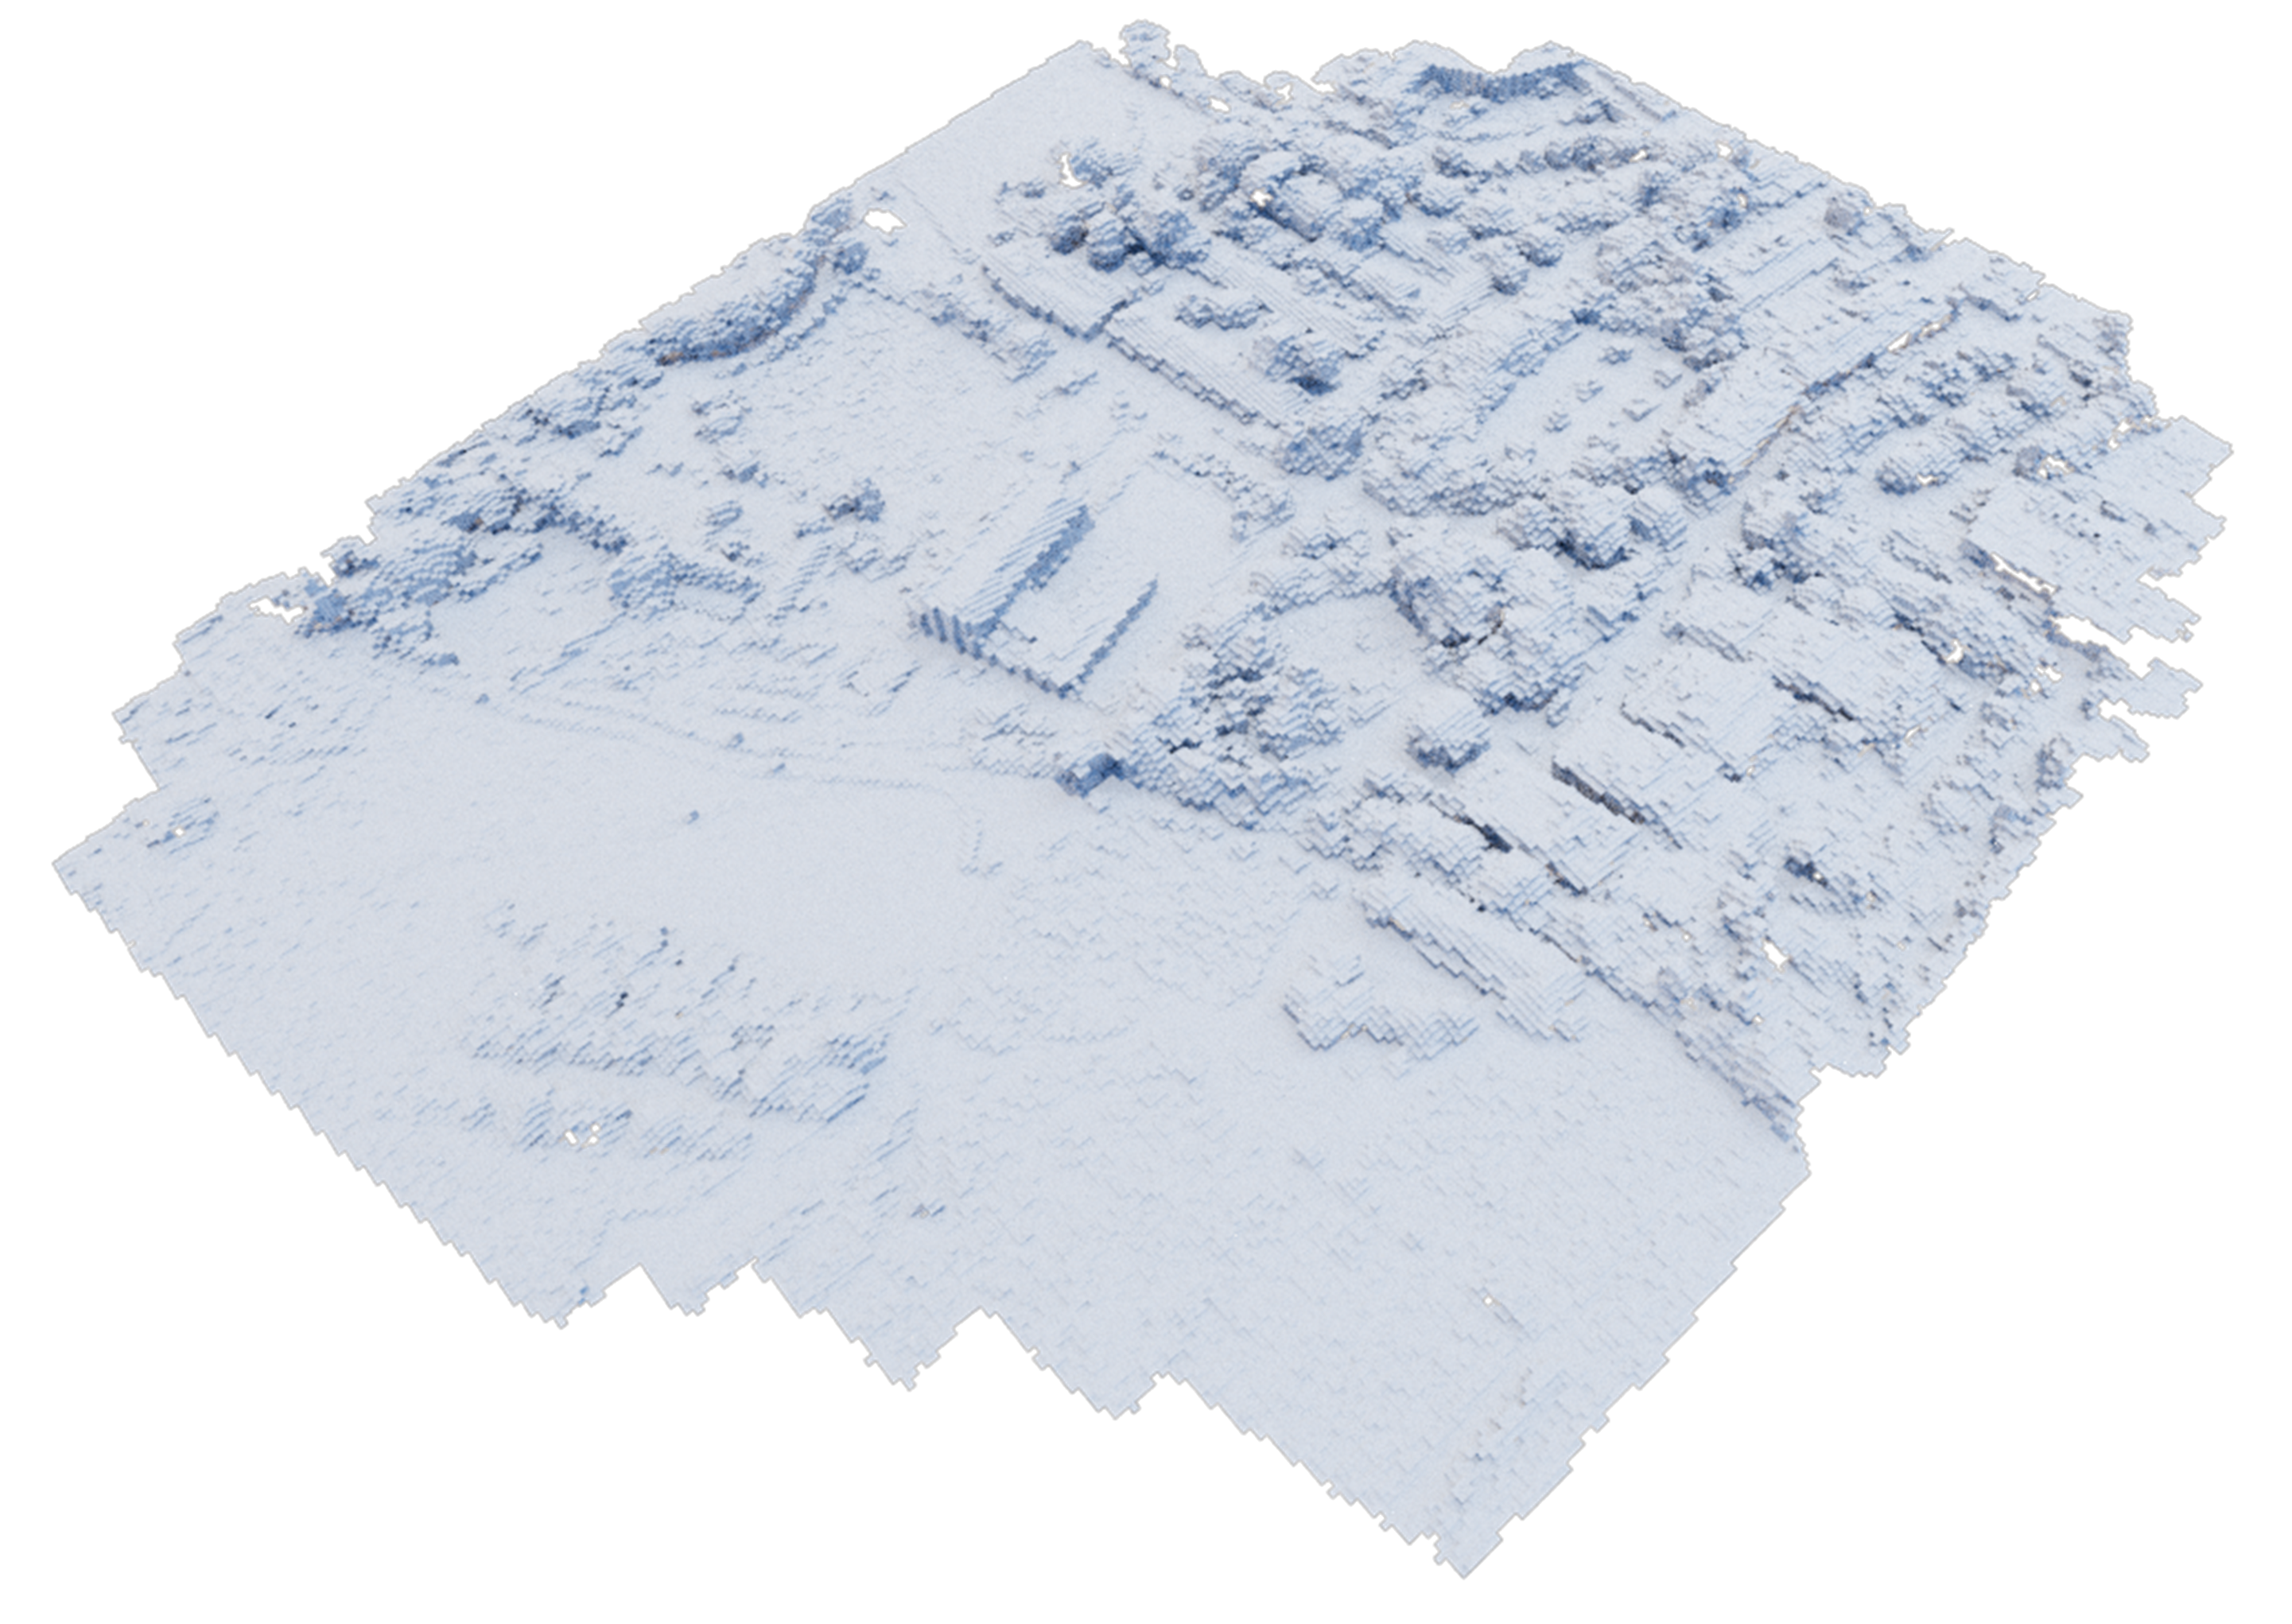
\includegraphics[width=\linewidth]{figs/hyper_point_cloud/voxelization.png}
	\caption{2.5D voxelization of an \acrshort{rgb} point cloud. }
	\label{fig:hyper_voxelization}
\end{marginfigure}
Points are processed in the \acrshort{gpu} using their height and index within a point cloud batch. The selection of the point with the highest altitude is implemented through an atomic block operating with \verb|uint64_t| values. The first 32 bits represent the altitude ($h$) and the least significant bits store the point index. Although $h \in \mathbb{R}$, it can be transformed into $h \in \mathbb{N}$ with \verb|floatBitsToInt| using its bit-level representation. Hence, the \verb|atomicMax| operator selects the highest altitude while it also carries the index. The result is a buffer that stores the indices of those points which are visible from hyperspectral swaths. From this stage, the hyperspectral point cloud can be straightforwardly computed by transferring hyperspectral layers as textures that can be sampled in the \acrshort{gpu}. However, note that large \acrshort{rgb} point clouds are downsampled according to the hyperspectral resolution. For instance, a point cloud of 330M points was narrowed to 17.5M points with a hyperspectral's \acrshort{gsd} of 0.067 \si{\meter}. Also, the dimensionality of the \acrshort{rgb} point cloud is further reduced since some \acrshort{rgb} points are not visible in hyperspectral data. This scenario occurs when the sampled texture coordinates, $u, v$, are not in $\left[0, 1\right]$, or invalid colours are sampled from the hyperspectral orthomosaic ($\alpha < 1$). The latter is derived from the computed orthomosaic being stored as a rectangular texture, where background pixels are marked using the alpha channel ($\alpha \gets 0$). 

\section{Hyperspectral data compression}

The main drawback of this projection approach is the large dimensionality of hyperspectral point clouds despite being downsampled, especially for \acrshort{gpu}-based buffers with a very limited capacity. In this work, a 2.5D hyperspectral point cloud of 17.5M points with 270 layers was represented with \verb|uint8_t| data type, which yields a total memory footprint of 4.4 GB. The compression and feature selection/transformation of hyperspectral datasets have been widely studied for reducing its footprint \cite{barrios_shyloc_2020, barrios_performance_2022} and extracting the most relevant features \cite{xuan_early_2022}. Regarding compression algorithms, there exist lossless approaches for hypercubes, though the data recovery is not as straightforward as in the representation proposed by Graciano et al. \cite{graciano_quadstack_2021}. For instance, the CSDS-123 \cite{barrios_shyloc_2020, barrios_performance_2022} is a standard algorithm to reduce the size of multispectral and hyperspectral data used in onboard satellites and military drones. Although it has been accelerated in the \acrshort{gpu} \cite{ferraz_hyperspectral_2021}, it is not aimed at providing a real-time readable data representation.

\begin{marginfigure}[-1.0cm]
    \centering
    \includegraphics[width=\linewidth]{figs/hyper_point_cloud/pavia_dataset.png}
	\caption{The 70th layer of the Pavia University hypercube. }
	\label{fig:hyper_pavia_dataset}
\end{marginfigure}
Despite hypercubes having a large number of changes throughout the spectral dimension, layers can be significantly compressed if their radiometric resolution is narrowed to the interval $\left[0, 2^8\right[$. Then, the hyperspectral point cloud can be compressed using a stack-based representation, as proposed by Graciano et al. \cite{graciano_quadstack_2021}, thus exploiting the similarity of surrounding layers in the $Z$-axis, i.e., the spectral signatures (Figure \ref{fig:hyper_compression_stack}). With this stack-based approach, the heightfield is first composed of $n$ voxels, determined by the number of points visible from $\textit{nadir}$ hyperspectral viewpoints. Then, these $n$ voxels are compacted by fusing layers that store the radiance (1 byte) and the number of consecutive layers with such a radiance value (2 bytes, as the number of layers in one pixel may be above $2^8$). Therefore, the compact layer representation requires 32 bits (\verb|uint32_t|) split as follows: number of layers (16 bits) and grayscale radiance (rest, 16 bits).

\begin{figure}[ht]
    \centering
    \includegraphics[width=.65\linewidth]{figs/hyper_point_cloud/stack.png}
	\caption{Stack-based representation for a hypercube with two layers. Only the first column is represented in the compact buffer. }
	\label{fig:hyper_compression_stack}
\end{figure}

Although this stack-based structure compressed the hypercube, its encoding presents a larger memory footprint (32 bits) in comparison with the initial 8 bits. Therefore, this approach is backed up by a significant compression that reduces the allocated memory albeit having a larger footprint per primitive. To prove that, this compression algorithm was tested against publicly available hypercubes \cite{noauthor_hyperspectral_nodate} as well as the proposed dataset, obtaining the following compression ratio: ours (39.77\%), Pavia Centre (56.74\%; Figure \ref{fig:hyper_pavia_dataset}), Pavia University (53.93\%), Kennedy Space Center (97.70\%), Salinas Valley (47.12\%) and Cuprite (59.20\%) datasets. Similarly to previous chapters, large point clouds do not fit in a single \acrshort{ssbo} and must be split into several batches, whose size depends on the data structure representation, the maximum number of layers and the allocatable memory. This dimensionality is calculated prior to compression as stated in Equation \ref{eq:maximum_hyper_batch_size}:
\begin{equation}
    n_{\textit{points}} = \lfloor{\frac{\max_{\mathtt{gpu\_bytes}}}{\mathtt{sizeof(uint32\_t)} * \mathtt{\max_{\mathtt{layers}}}}\rfloor}
    \label{eq:maximum_hyper_batch_size}
\end{equation}

\subsection{Point cloud rendering}

The visualization of hyperspectral point clouds is relevant as it enables visual inspections and band-wise rendering. To tackle the lack of density that may affect hyperspectral point clouds, these have been rendered using \acrshort{opengl}'s compute shaders. To this end, the approach of Schütz et al. \cite{schutz_rendering_2021} was followed, obtaining results such as the one depicted in Figure \ref{fig:hyper_hqs_optimization}. The point cloud was sorted according to the 3D Morton encoding with 30 bits, and batches of small size were shuffled to avoid load unbalancing in the \acrshort{gpu}. Nevertheless, red and green channels were discarded during the accumulation stage of this procedure; instead, only the blue (radiance) and $\alpha$ (number of points) channels were used. 

\begin{marginfigure}[.cm]
    \centering
    \includegraphics[width=\linewidth]{figs/hyper_point_cloud/hqs_optimization.png}
	\caption{Rendering of a point cloud with the Green wavelength, using the optimization described by Schütz et al. \cite{schutz_rendering_2021}. }
	\label{fig:hyper_hqs_optimization}
\end{marginfigure}
Colours are retrieved by traversing stacks from the described compression data structure, evaluating the target layer as well as the number of repeats per stack layer. The main concern in the rendering is the frame rate for the last stacks, as the traversal time is higher and loops are very inefficient in shaders. To tackle this, images are iteratively constructed in multiple frames instead of a single one, thus reducing the latency of single frames. The user visualizes an incomplete, yet sufficient, point cloud that helps to find the better camera location until the image is fully constructed in a few frames. A noise buffer $N$, where $N \in \mathbf{N}^k, N_i \in \left[0, n_{\textit{points}}\right[$ and $n_{\textit{points}}$ is the number of points, indicates which points are rendered in every frame. It can be shifted in subsequent frames to render every visible point and converge into a fully rendered image. The number of frames required to converge depends on the buffer length, $k$. Finally, Figure \ref{fig:hyper_iterative_rendering} shows several stages of progressive rendering.

\begin{figure*}[ht]
    \centering
    \includegraphics[width=\linewidth]{figs/hyper_point_cloud/iterative_rendering.png}
	\caption{Iterative rendering of a hyperspectral point cloud during several frames, using 10k points per frame.}
	\label{fig:hyper_iterative_rendering}
\end{figure*}

\section{Results and discussion}

The performance of the proposed method has been evaluated using point clouds and images of different sizes. The baseline \acrshort{rgb} point cloud is generated with two different numbers of points, 150M and 330M, while other subsampled point clouds will be used for further assessing the performance. Due to the lack of previous work concerning the generation of 3D hyperspectral point clouds, this section is solely focused on the performance of individual stages, from the generation of hyperspectral orthomosaics to data compression and rendering. The reported results are obtained as the average from five different executions.

Measurements were performed on a PC with Intel Core i7-7700 3.6 GHz, 16 GB RAM, NVIDIA GTX 1070 \acrshort{gpu} with 8 GB \acrshort{vram} (Pascal architecture), and Windows 10 \acrshort{os}. The proposed methodology is implemented in C++ along with \acrshort{opengl}. Massively parallel processes were developed in \acrshort{glsl} using general-purpose compute shaders, whereas \acrshort{cpu}-based methods are accelerated using the multi-threading \acrshort{openmp} library.

\subsection{Study area and data acquisition}

The study area is located at the University of Trás-os-Montes e Alto Douro campus, covering 4 \si{\hectare}. Its altitude is 500 \si{\meter}, though it varies up to 30 \si{\meter} in the surveyed area. \acrshort{gcp}s were uniformly distributed to provide high positional accuracy in contrast to the \acrshort{uas}’s \acrshort{gnss} receiver. Therefore, the collected images were georeferenced using five \acrshort{gcp}s depicted as circular targets with a diameter of size 0.5 \si{\meter}. Besides \acrshort{gcp}s, control points were also used to assess the quality of the results. Both \acrshort{gcp}s and \acrshort{cp}s were measured with a \acrshort{gnss} receiver based on the TM06/ETRS89 coordinate system.

Hyperspectral swaths were collected with 40\% side overlap at an altitude of 100 \si{\meter}, thus acquiring 6 different hyperspectral images. The \acrshort{rgb} dataset is composed of 324 \acrshort{rgb} images acquired with a spatial resolution of 3.4 \si{\centi\meter}, 90\% frontal overlap and 75\% side overlap at an altitude of 80 \si{\meter} from the take-off position. The latter is processed with Pix4Dmapper to obtain the baseline \acrshort{rgb} point clouds. 

\subsection{Performance analysis}

The performance is assessed for every stage against a sequential approach. Firstly, hyperspectral images were aggregated to compute the hyperspectral orthomosaic. Although hyperspectral swaths have a limited resolution, the stitching procedure from Jurado et al. \cite{jurado_efficient_2022} generates a large hyperspectral orthomosaic. Hence, the response time has been assessed for different image resolutions by upscaling and downscaling the collected swaths. As shown in Figure \ref{fig:hyper_aggregation_results}, the response time was very reduced even for upscaled imagery (2x, 4x) despite this process being repeated once for every hyperspectral layer. Thus, the aggregation was solved in 130 \si{\milli\second} for a single layer using the starting resolution, whereas the half-size setup achieved a significant speedup (74.69\%). The aggregation stage is the main bottleneck since it comprises multiple operators. On the other hand, the allocation and reading phases had a higher response time as a result of transferring large buffers between \acrshort{cpu} and \acrshort{gpu}. Regarding the \acrshort{cpu} versus \acrshort{gpu} comparison, the speedup of the second approach is 92.54\%.

\begin{figure*}[bt]
    \centering
    \includegraphics[width=\linewidth]{figs/hyper_point_cloud/hyper_aggregation_performance.png}
    \caption{Response time in \si{\milli\second} for the \acrshort{gpu}-based approach, stacked per aggregation stage, whereas the chart in the right side compares the performance of both \acrshort{cpu} and \acrshort{gpu}-based methods.}
    \label{fig:hyper_aggregation_results}
\end{figure*}

After the orthomosaic generation, the point cloud is voxelized as a heightfield to obtain which points are visible according to their height within a voxel. Hence, Figure \ref{fig:hyper_voxelization_results} shows the response time for building heightfields over point clouds of different dimensionality. The resolution varies from 0.02 \si{\meter} to 2 \si{\meter}, including the default hyperspectral resolution (0.067 \si{\meter}). Measurements integrate both the allocation stage and the thread logic. Although input point clouds are very large, the voxelization was efficiently solved in the \acrshort{gpu} using a single atomic operation for points projected in a voxel. It was solved in 500 \si{\milli\second} since the processing is performed for each point regardless of the resolution. In contrast to the \acrshort{gpu} approach, the sequential algorithm notably increased the latency for larger point clouds (+96.66\% for 330M points).

\begin{figure}[bt]
    \centering
    \includegraphics[width=\linewidth]{figs/hyper_point_cloud/voxelization_results.png}
	\caption{Performance of 2.5D voxelization for three different point clouds. Dotted lines show the results of the \acrshort{cpu}-based approach, while solid lines represent the \acrshort{gpu}-accelerated one. }
	\label{fig:hyper_voxelization_results}
\end{figure}

Then, the projection and compression stages are performed using the visible points and the previously stitched orthomosaic. Figure \ref{fig:hyper_compression_results} shows the response time for building a hyperspectral point cloud and compressing it. To this end, this procedure was evaluated using four point clouds with a size ranging from 15M to 330M, whereas the heightfield was constructed with a resolution equal to the \acrshort{gsd} from hyperspectral data. Larger point clouds obtained a higher compression rate as they also had higher density and a larger number of voxels, with some of them showing little variance in the spectral dimension. The response time ranged from 5 \si{\second} for 15M points to 80 \si{\second} for 330M points. Hence, the first point cloud was compressed by iterating through a few point cloud subdivisions, whereas the last one requires over fifty subdivisions. Hyperspectral images were iteratively used for each subdivision, though its transferring time is mitigated by building a large buffer composed of the whole set of layers instead of uploading each one multiple times. Therefore, the initial delay is significantly higher, though it provides a speedup in comparison with a continuous data stream to the \acrshort{gpu}. The speedup of \acrshort{gpu}-based approaches in contrast to \acrshort{cpu} is considerably higher in this stage since it involves multiple iterations. Accordingly, the improvement ranges from 96.59\% (15M) to 99.35\% (330M).

\begin{figure}[bt]
    \centering
    \includegraphics[width=\linewidth]{figs/hyper_point_cloud/compression_results.png}
	\caption{Response time (\si{\second}) for building a hyperspectral point cloud with 270 spectral bands. }
	\label{fig:hyper_compression_results}
\end{figure}

Finally, the frame rate for rendering the hyperspectral point cloud is shown in Figure \ref{fig:hyper_fps_performance}. The target layer is iteratively increased for each new frame over two point clouds of size 150M and 330M. On the other hand, activations refer to the length of the noise buffer, thus referring to the maximum number of points rendered per frame. In this regard, two different activation values were used: 5k and 10k per frame. As depicted, the main drawback of stack-based compression is the traversal of the data structure to retrieve the original data, since deeper target layers also involve a larger number of iterations and response time. However, a lower activation size reduces the response time derived from constructing a single frame, whereas the complete scenario is generated in a reduced time. Finally, the number of point cloud subdivisions also worsens the performance since it increases the number of compute shader calls. Note that even the first layers are affected by the latter drawback. 

\begin{figure}[bt]
    \centering
    \includegraphics[width=\linewidth]{figs/hyper_point_cloud/hyper_fps_results.png}
	\caption{Frame rate for rendering hyperspectral point clouds with an increasing target layer. Activations refer to the number of points which were rendered in every frame. }
	\label{fig:hyper_fps_performance}
\end{figure}

\section{Conclusions and future work}

In this work, a method for the efficient generation of hyperspectral point clouds has been proposed. According to the limitations of hyperspectral acquisition, the collected swaths were first stitched to construct a large hyperspectral orthomosaic. Then, it was projected into the voxelization of an \acrshort{rgb} point cloud, thereby constructing a 2.5D hyperspectral point cloud. The resulting heightfield was compressed with a stack-based representation and rendered iteratively to enhance the visualization performance. The whole pipeline was implemented in the \acrshort{gpu}, thus showing speedups over 90\% in comparison with the \acrshort{cpu}-based stages, even for sparse point clouds (15M points).

As a future work, the rendering pipeline could be further improved together with the stack-based compressed data, mainly addressing the traversal time in compute shaders. Also, \acrshort{gpu} buffers allocated for the hypercube could be further compacted, maybe exploring other efficient compression approaches, to reduce the number of point cloud subdivisions and the allocated \acrshort{gpu}'s memory. 

\begin{kaobox}[frametitle=Compression of spatial data from hypercubes with QuadStack]
The QuadStack compression method proposed by Graciano et al. \cite{graciano_quadstack_2021} also operates in the spatial dimensions, although the used datasets were further stressed in this regard and they showed a poor performance. Hence, spectral compression was proven to be possible with a lower radiometric resolution, whereas spatial compression does not work well with this approach.  
\end{kaobox}